\documentclass{beamer}
\usepackage[utf8]{inputenc}
\usepackage[T1]{fontenc}
\usepackage[UKenglish]{babel}
\usepackage[UKenglish]{isodate}
\usepackage{graphicx}
\usepackage[style=authoryear]{biblatex}
\usepackage{tikz}
\usepackage{empheq}
\usepackage{dashbox}
\usepackage{complexity}

\usetheme{Amsterdam}
\beamertemplatenavigationsymbolsempty
\addbibresource{../review.bib}
\newtheorem{conjecture}{Conjecture}

\usetikzlibrary{decorations.pathreplacing}
\usetikzlibrary{arrows.meta}
\usetikzlibrary{cd}
\tikzstyle{na} = [baseline=-0.5ex]
\tikzstyle{every picture}+=[remember picture]

\DeclareMathOperator{\ifff}{:-}
\DeclareMathOperator{\prob}{::}
\definecolor{color1}{HTML}{1b9e77}
\definecolor{color2}{HTML}{d95f02}
\definecolor{color3}{HTML}{7570b3}
\definecolor{color4}{HTML}{e7298a}
\definecolor{color5}{HTML}{66a61e}
\definecolor{color6}{HTML}{e6ab02}
\definecolor{color7}{HTML}{e9eff4}

\author{Paulius Dilkas}
\title{Foundations for Inference in Probabilistic Relational Models}

\begin{document}

\maketitle

%\begin{frame}{Outline}
%  \tableofcontents
%\end{frame}

\AtBeginSection[]
{
  \begin{frame}<beamer>
    \frametitle{Outline}
    \tableofcontents[currentsection]
  \end{frame}
}

\section{Introduction}

\begin{frame}{Probabilistic Relational Models}
  \begin{block}{Markov Logic Network (\cite{DBLP:journals/ml/RichardsonD06})}
    \vspace*{-\baselineskip}\setlength\belowdisplayshortskip{0pt}
    \begin{align*}
      0.7 &\quad \forall x \forall y \forall z \; \mathtt{Friends}(x, y) \land \mathtt{Friends}(y, z) \Rightarrow \mathtt{Friends}(x, z) \\
      2.3 &\quad \forall x \; \lnot\exists y \; \mathtt{Friends}(x, y) \Rightarrow \mathtt{Smokes}(x) \\
      1.5 &\quad \forall x \; \mathtt{Smokes}(x) \Rightarrow \mathtt{Cancer}(x) \\
      1.1 &\quad \forall x \forall y \; \mathtt{Friends}(x, y) \Rightarrow (\mathtt{Smokes}(x) \Leftrightarrow \mathtt{Smokes}(y))
    \end{align*}
  \end{block}
\end{frame}

\begin{frame}{Probabilistic Relational Models}
  \begin{block}{ProbLog (\cite{DBLP:conf/ijcai/RaedtKT07})}
    \vspace*{-\baselineskip}\setlength\belowdisplayshortskip{0pt}
    \begin{align*}
      1.0 &\prob \mathtt{likes}(X, Y) \ifff \mathtt{friendOf}(X, Y). \\
      0.8 &\prob \mathtt{likes}(X, Y) \ifff \mathtt{friendOf}(X, Z), \mathtt{likes}(Z, Y). \\
      0.5 &\prob \mathtt{friendOf}(\mathit{john}, \mathit{mary}). \\
      0.5 &\prob \mathtt{friendOf}(\mathit{mary}, \mathit{pedro}). \\
      0.5 &\prob \mathtt{friendOf}(\mathit{mary}, \mathit{tom}). \\
      0.5 &\prob \mathtt{friendOf}(\mathit{pedro}, \mathit{tom}).
    \end{align*}
  \end{block}
\end{frame}

\begin{frame}{Probabilistic Relational Models}
  \begin{itemize}
  \item What do these models have in common?
  \item When performing inference...
    \begin{itemize}
    \item do we have to consider every detail?
    \item what makes inference challenging?
    \item can we do any better?
    \end{itemize}
  \item How can we learn PRMs from data?
  \end{itemize}
\end{frame}

\begin{frame}{Applications}
  \begin{columns}
    \begin{column}{0.5\textwidth}
      \centering
      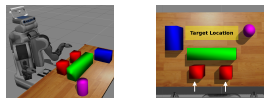
\includegraphics[width=\textwidth,height=0.5\textheight,keepaspectratio]{application_robots.jpg}
      \\[-7pt]
      {\tiny \cite{DBLP:conf/iros/MoldovanR14}}
      \vfill
      \null
      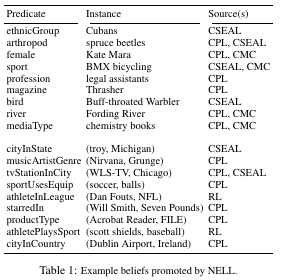
\includegraphics[width=\textwidth,height=0.5\textheight,keepaspectratio]{application_nell.jpg}
      \\[-7pt]
      {\tiny \cite{DBLP:conf/aaai/CarlsonBKSHM10}}
    \end{column}
    \begin{column}{0.5\textwidth}
      \centering
      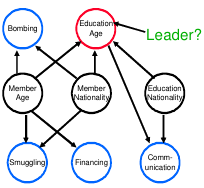
\includegraphics[width=\textwidth,height=0.4\textheight,keepaspectratio]{application_criminal.jpg}
      \\[-7pt]
      {\tiny \cite{DBLP:conf/sdm/DelaneyFCWJ10}}
      \vfill
      \null
      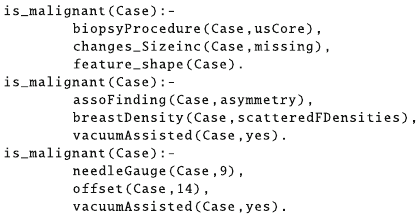
\includegraphics[width=\textwidth,height=0.5\textheight,keepaspectratio]{application_cancer.jpg}
      \\[-7pt]
      {\tiny \cite{DBLP:conf/ilp/Corte-RealD017}}
    \end{column}
  \end{columns}
\end{frame}

\section{Equivalence}

\begin{frame}
  \begin{columns}
    \begin{column}{0.5\textwidth}
      \begin{alertblock}{}
        \vspace*{-1.5\baselineskip}\setlength\belowdisplayshortskip{0pt}
        \begin{gather*}
          \mathtt{Husband}(\mathit{joffrey}, \mathit{margaery}) \\
          \mathtt{Husband}(\mathit{tommen}, \mathit{margaery}) \\
          \mathtt{Husband}(\mathit{renly}, \mathit{margaery}) \\
          \mathtt{Parent}(\mathit{cersei}, \mathit{joffrey}) \\
          \mathtt{Parent}(\mathit{cersei}, \mathit{myrcella}) \\
          \mathtt{Parent}(\mathit{cersei}, \mathit{tommen}) \\
          \mathtt{Parent}(\mathit{tywin}, \mathit{cersei})
        \end{gather*}
        \vspace*{-1.5\baselineskip}\setlength\belowdisplayshortskip{0pt}
      \end{alertblock}
    \end{column}
    \begin{column}{0.5\textwidth}
      \begin{exampleblock}{}<2->
        \vspace*{-1.5\baselineskip}\setlength\belowdisplayshortskip{0pt}
        \begin{gather*}
          \mathtt{Female}(\mathit{cersei}), \\
          \mathtt{Female}(\mathit{margaery}), \\
          \mathtt{Female}(\mathit{myrcella})
        \end{gather*}
        \vspace*{-1.5\baselineskip}\setlength\belowdisplayshortskip{0pt}
      \end{exampleblock}
    \end{column}
  \end{columns}
  \begin{block}{}<3->
    \vspace*{-1.5\baselineskip}\setlength\belowdisplayshortskip{0pt}
    \begin{align*}
      \mathtt{Female}(X) &\ifff \mathtt{Husband}(\mathit{joffrey}, X). \\
      \mathtt{Female}(X) &\ifff \mathtt{Parent}(X, \mathit{joffrey}). \\
      \mathtt{Female}(X) &\ifff \mathtt{Parent}(\mathit{cersei}, X), \neg\mathtt{Husband}(X, \mathit{margaery}).
    \end{align*}
    \vspace*{-1.5\baselineskip}\setlength\belowdisplayshortskip{0pt}
  \end{block}
\end{frame}

\begin{frame}{Main Results}
  \begin{definition}[Equivalence]
    Two $n$-tuples of constants $a$ and $b$ are \alert{equivalent} if
    \[
      (\mathtt{P} \circ \rho)(a) = (\mathtt{P} \circ \rho)(b)
    \]
    for all atoms $\mathtt{P} \circ \rho$ acting on $n$ variables.
  \end{definition}
  \pause
  \begin{theorem}
    There is a logic program $\mathcal{L}\colon \mathcal{KB}(P_1, C) \to
    \mathcal{KB}(P_2, C)$ such that $\mathcal{L}(\Delta_1) = \Delta_2$ if and
    only if ${\sim_{\Delta_2}}$ is coarser than ${\sim_{\Delta_1}}$.
  \end{theorem}
\end{frame}

\section{Random Programs}

\begin{frame}{What Characterises a Program?}
  \begin{columns}
    \hspace*{-0.7cm}\begin{column}{0.75\textwidth}
      \begin{empheq}[left =\onslide<6->{\color{color5}\empheqlbrace}]{equation}
        \begin{align*}
          \textcolor<5->{color4}{1.0} &\prob \textcolor<2->{color1}{\mathtt{likes}}(\textcolor<3->{color2}{X}, \textcolor<3->{color2}{Y}) \ifff \textcolor<2->{color1}{\mathtt{friendOf}}(\textcolor<3->{color2}{X}, \textcolor<3->{color2}{Y}). \\
          \textcolor<5->{color4}{0.8} &\prob \textcolor<2->{color1}{\mathtt{likes}}(\textcolor<3->{color2}{X}, \textcolor<3->{color2}{Y}) \ifff \tikz \coordinate (start);\textcolor<2->{color1}{\mathtt{friendOf}}(\textcolor<3->{color2}{X}, \textcolor<3->{color2}{Z}), \textcolor<2->{color1}{\mathtt{likes}}(\textcolor<3->{color2}{Z}, \textcolor<3->{color2}{Y})\tikz \coordinate (end);. \\
          \textcolor<5->{color4}{0.5} &\prob \textcolor<2->{color1}{\mathtt{friendOf}}(\textcolor<4->{color3}{\mathit{john}}, \textcolor<4->{color3}{\mathit{mary}}). \\
          \textcolor<5->{color4}{0.5} &\prob \textcolor<2->{color1}{\mathtt{friendOf}}(\textcolor<4->{color3}{\mathit{mary}}, \textcolor<4->{color3}{\mathit{pedro}}). \\
          \textcolor<5->{color4}{0.5} &\prob \textcolor<2->{color1}{\mathtt{friendOf}}(\textcolor<4->{color3}{\mathit{mary}}, \textcolor<4->{color3}{\mathit{tom}}). \\
          \textcolor<5->{color4}{0.5} &\prob \textcolor<2->{color1}{\mathtt{friendOf}}(\textcolor<4->{color3}{\mathit{pedro}}, \textcolor<4->{color3}{\mathit{tom}}).
        \end{align*}
      \end{empheq}
    \end{column}
    \begin{column}{0.25\textwidth}
      \begin{itemize}
      \item[\textcolor{color1}{\textbullet}]<2-> predicates, arities
      \item[\textcolor{color2}{\textbullet}]<3-> variables
      \item[\textcolor{color3}{\textbullet}]<4-> constants
      \item[\textcolor{color4}{\textbullet}]<5-> probabilities
      \item[\textcolor{color5}{\textbullet}]<6-> length
      \item[\textcolor{color6}{\textbullet}]<7-> complexity
      \end{itemize}
    \end{column}
  \end{columns}
  \onslide<7->{
    \begin{tikzpicture}[overlay]
      \draw [decorate,decoration={brace,amplitude=10pt,mirror},color=color6] (start) -- (end);
    \end{tikzpicture}
  }
  \begin{columns}
    \begin{column}{0.27\textwidth}
      \onslide<9->{
        Also:
        \begin{itemize}
        \item cyclicity
        \item (conditional) independence
        \item required subformulas
        \end{itemize}
      }
    \end{column}
    \begin{column}{0.53\textwidth}
      \onslide<8->{
        \begin{tikzpicture}
          \node[draw,circle,gray,text=black] (and) at (0, 0) {$\land$};
          \node[draw,gray,text=black] (friendOf) at (-1.5, -1) {$\textcolor{color1}{\mathtt{friendOf}}\textcolor{black}{(}\textcolor<3->{color2}{X}\textcolor{black}{,}\,\textcolor<3->{color2}{Z}\textcolor{black}{)}$};
          \node[draw,gray,text=black] (likes) at (1.5, -1) {$\textcolor{color1}{\mathtt{likes}}\textcolor{black}{(}\textcolor<3->{color2}{Z}\textcolor{black}{,}\,\textcolor<3->{color2}{Y}\textcolor{black}{)}$};
          \draw[gray] (and) -- (friendOf);
          \draw[gray] (and) -- (likes);
        \end{tikzpicture}
      }
    \end{column}
    \begin{column}{0.2\textwidth}
      \onslide<10->{
        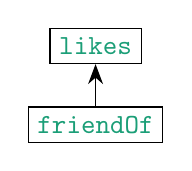
\begin{tikzpicture}
          \node[draw] (likes) {\textcolor{color1}{$\mathtt{likes}$}};
          \node[draw,below of = likes] (friendOf) {\textcolor{color1}{$\mathtt{friendOf}$}};
          \draw[-{Stealth[scale=1.5]}] (friendOf) -- (likes);
        \end{tikzpicture}
      }
    \end{column}
  \end{columns}
\end{frame}

\begin{frame}{What Programs Are Hard to Generate?}
  \begin{figure}
    \centering
    % Created by tikzDevice version 0.12.3.1 on 2022-06-27 14:20:09
% !TEX encoding = UTF-8 Unicode
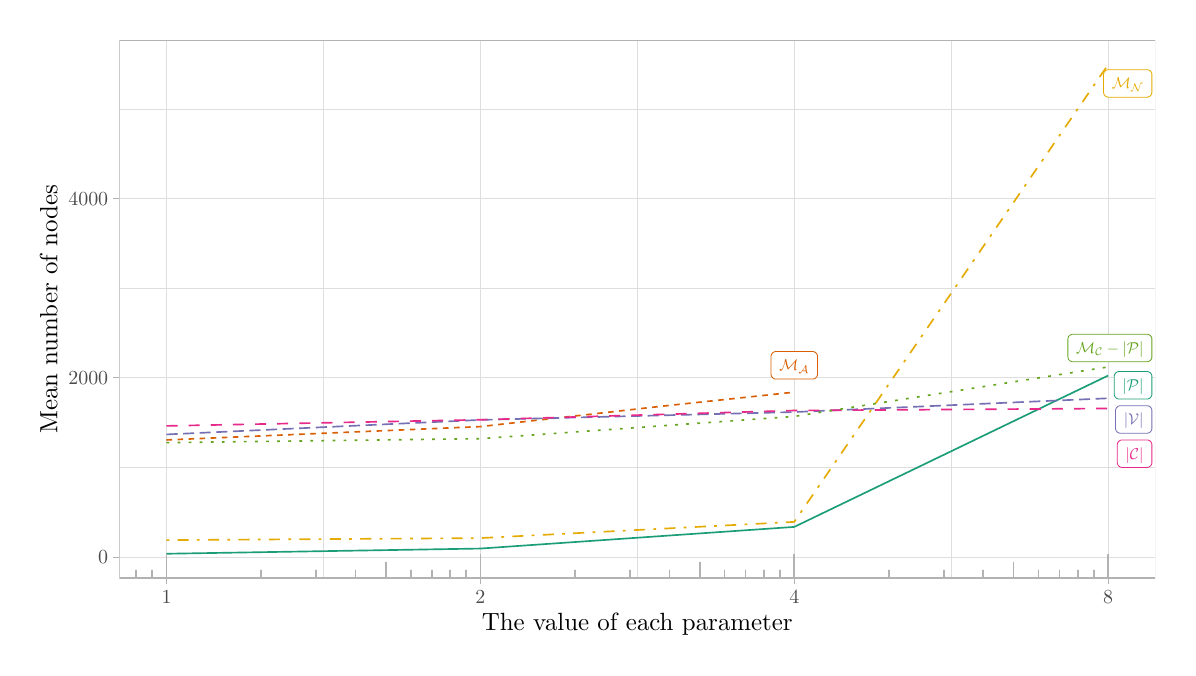
\begin{tikzpicture}[x=1pt,y=1pt]
\definecolor{fillColor}{RGB}{255,255,255}
\path[use as bounding box,fill=fillColor,fill opacity=0.00] (0,0) rectangle (411.94,224.04);
\begin{scope}
\path[clip] (  0.00,  0.00) rectangle (411.94,224.04);
\definecolor{drawColor}{RGB}{255,255,255}
\definecolor{fillColor}{RGB}{255,255,255}

\path[draw=drawColor,line width= 0.5pt,line join=round,line cap=round,fill=fillColor] (  0.00,  0.00) rectangle (411.94,224.04);
\end{scope}
\begin{scope}
\path[clip] ( 33.14, 25.11) rectangle (407.44,219.54);
\definecolor{fillColor}{RGB}{255,255,255}

\path[fill=fillColor] ( 33.14, 25.11) rectangle (407.44,219.54);
\definecolor{drawColor}{gray}{0.87}

\path[draw=drawColor,line width= 0.1pt,line join=round] ( 33.14, 65.17) --
	(407.44, 65.17);

\path[draw=drawColor,line width= 0.1pt,line join=round] ( 33.14,129.92) --
	(407.44,129.92);

\path[draw=drawColor,line width= 0.1pt,line join=round] ( 33.14,194.66) --
	(407.44,194.66);

\path[draw=drawColor,line width= 0.1pt,line join=round] (106.87, 25.11) --
	(106.87,219.54);

\path[draw=drawColor,line width= 0.1pt,line join=round] (220.29, 25.11) --
	(220.29,219.54);

\path[draw=drawColor,line width= 0.1pt,line join=round] (333.71, 25.11) --
	(333.71,219.54);

\path[draw=drawColor,line width= 0.2pt,line join=round] ( 33.14, 32.80) --
	(407.44, 32.80);

\path[draw=drawColor,line width= 0.2pt,line join=round] ( 33.14, 97.54) --
	(407.44, 97.54);

\path[draw=drawColor,line width= 0.2pt,line join=round] ( 33.14,162.29) --
	(407.44,162.29);

\path[draw=drawColor,line width= 0.2pt,line join=round] ( 50.16, 25.11) --
	( 50.16,219.54);

\path[draw=drawColor,line width= 0.2pt,line join=round] (163.58, 25.11) --
	(163.58,219.54);

\path[draw=drawColor,line width= 0.2pt,line join=round] (277.00, 25.11) --
	(277.00,219.54);

\path[draw=drawColor,line width= 0.2pt,line join=round] (390.43, 25.11) --
	(390.43,219.54);
\definecolor{drawColor}{RGB}{27,158,119}

\path[draw=drawColor,line width= 0.6pt,line join=round] ( 50.16, 33.94) --
	(163.58, 35.82) --
	(277.00, 43.64) --
	(390.43, 98.33);
\definecolor{drawColor}{RGB}{217,95,2}

\path[draw=drawColor,line width= 0.6pt,dash pattern=on 2pt off 2pt ,line join=round] ( 50.16, 75.06) --
	(163.58, 79.89) --
	(229.93, 87.34) --
	(277.00, 92.33);
\definecolor{drawColor}{RGB}{117,112,179}

\path[draw=drawColor,line width= 0.6pt,dash pattern=on 4pt off 2pt ,line join=round] ( 50.16, 77.05) --
	(163.58, 82.31) --
	(277.00, 85.14) --
	(390.43, 90.12);
\definecolor{drawColor}{RGB}{231,41,138}

\path[draw=drawColor,line width= 0.6pt,dash pattern=on 4pt off 4pt ,line join=round] ( 50.16, 80.14) --
	(163.58, 82.36) --
	(277.00, 85.70) --
	(390.43, 86.43);
\definecolor{drawColor}{RGB}{102,166,30}

\path[draw=drawColor,line width= 0.6pt,dash pattern=on 1pt off 3pt ,line join=round] ( 50.16, 74.09) --
	(163.58, 75.52) --
	(277.00, 83.56) --
	(390.43,101.45);
\definecolor{drawColor}{RGB}{230,171,2}

\path[draw=drawColor,line width= 0.6pt,dash pattern=on 1pt off 3pt on 4pt off 3pt ,line join=round] ( 50.16, 38.87) --
	(163.58, 39.60) --
	(277.00, 45.46) --
	(390.43,210.70);
\end{scope}
\begin{scope}
\path[clip] ( 33.14, 25.11) rectangle (407.44,219.54);

\path[] (399.52, 75.07) -- (390.90, 85.83);
\definecolor{drawColor}{RGB}{27,158,119}
\definecolor{fillColor}{RGB}{255,255,255}

\path[draw=drawColor,line width= 0.3pt,line join=round,line cap=round,fill=fillColor] (394.43, 89.84) --
	(404.43, 89.84) --
	(404.35, 89.85) --
	(404.65, 89.86) --
	(404.93, 89.92) --
	(405.20, 90.02) --
	(405.45, 90.16) --
	(405.68, 90.35) --
	(405.87, 90.57) --
	(406.03, 90.81) --
	(406.14, 91.08) --
	(406.21, 91.36) --
	(406.23, 91.65) --
	(406.23, 91.65) --
	(406.23, 97.98) --
	(406.23, 97.98) --
	(406.21, 98.27) --
	(406.14, 98.55) --
	(406.03, 98.82) --
	(405.87, 99.06) --
	(405.68, 99.28) --
	(405.45, 99.47) --
	(405.20, 99.61) --
	(404.93, 99.71) --
	(404.65, 99.77) --
	(404.43, 99.79) --
	(394.43, 99.79) --
	(394.65, 99.77) --
	(394.36, 99.78) --
	(394.07, 99.75) --
	(393.79, 99.67) --
	(393.53, 99.54) --
	(393.29, 99.38) --
	(393.08, 99.18) --
	(392.90, 98.94) --
	(392.77, 98.69) --
	(392.68, 98.41) --
	(392.63, 98.12) --
	(392.62, 97.98) --
	(392.62, 91.65) --
	(392.63, 91.80) --
	(392.63, 91.51) --
	(392.68, 91.22) --
	(392.77, 90.94) --
	(392.90, 90.68) --
	(393.08, 90.45) --
	(393.29, 90.25) --
	(393.53, 90.09) --
	(393.79, 89.96) --
	(394.07, 89.88) --
	(394.36, 89.85) --
	cycle;
\end{scope}
\begin{scope}
\path[clip] ( 33.14, 25.11) rectangle (407.44,219.54);
\definecolor{drawColor}{RGB}{27,158,119}

\node[text=drawColor,anchor=base,inner sep=0pt, outer sep=0pt, scale=  0.57] at (399.43, 92.86) {$|\mathcal{P}|$};
\definecolor{drawColor}{RGB}{117,112,179}
\definecolor{fillColor}{RGB}{255,255,255}

\path[draw=drawColor,line width= 0.3pt,line join=round,line cap=round,fill=fillColor] (394.90, 77.50) --
	(404.43, 77.50) --
	(404.35, 77.50) --
	(404.65, 77.51) --
	(404.93, 77.57) --
	(405.20, 77.67) --
	(405.45, 77.82) --
	(405.68, 78.00) --
	(405.87, 78.22) --
	(406.03, 78.46) --
	(406.14, 78.73) --
	(406.21, 79.01) --
	(406.23, 79.30) --
	(406.23, 79.30) --
	(406.23, 85.63) --
	(406.23, 85.63) --
	(406.21, 85.92) --
	(406.14, 86.20) --
	(406.03, 86.47) --
	(405.87, 86.72) --
	(405.68, 86.94) --
	(405.45, 87.12) --
	(405.20, 87.26) --
	(404.93, 87.37) --
	(404.65, 87.43) --
	(404.43, 87.44) --
	(394.90, 87.44) --
	(395.12, 87.43) --
	(394.83, 87.44) --
	(394.54, 87.40) --
	(394.26, 87.32) --
	(394.00, 87.20) --
	(393.76, 87.03) --
	(393.55, 86.83) --
	(393.37, 86.60) --
	(393.24, 86.34) --
	(393.15, 86.06) --
	(393.10, 85.78) --
	(393.09, 85.63) --
	(393.09, 79.30) --
	(393.10, 79.45) --
	(393.10, 79.16) --
	(393.15, 78.87) --
	(393.24, 78.60) --
	(393.37, 78.34) --
	(393.55, 78.11) --
	(393.76, 77.90) --
	(394.00, 77.74) --
	(394.26, 77.61) --
	(394.54, 77.53) --
	(394.83, 77.50) --
	cycle;
\end{scope}
\begin{scope}
\path[clip] ( 33.14, 25.11) rectangle (407.44,219.54);
\definecolor{drawColor}{RGB}{117,112,179}

\node[text=drawColor,anchor=base,inner sep=0pt, outer sep=0pt, scale=  0.57] at (399.66, 80.51) {$|\mathcal{V}|$};
\definecolor{drawColor}{RGB}{231,41,138}
\definecolor{fillColor}{RGB}{255,255,255}

\path[draw=drawColor,line width= 0.3pt,line join=round,line cap=round,fill=fillColor] (395.53, 65.13) --
	(404.43, 65.13) --
	(404.35, 65.13) --
	(404.65, 65.14) --
	(404.93, 65.20) --
	(405.20, 65.30) --
	(405.45, 65.45) --
	(405.68, 65.63) --
	(405.87, 65.85) --
	(406.03, 66.09) --
	(406.14, 66.36) --
	(406.21, 66.64) --
	(406.23, 66.93) --
	(406.23, 66.93) --
	(406.23, 73.26) --
	(406.23, 73.26) --
	(406.21, 73.55) --
	(406.14, 73.83) --
	(406.03, 74.10) --
	(405.87, 74.35) --
	(405.68, 74.56) --
	(405.45, 74.75) --
	(405.20, 74.89) --
	(404.93, 75.00) --
	(404.65, 75.05) --
	(404.43, 75.07) --
	(395.53, 75.07) --
	(395.75, 75.05) --
	(395.46, 75.07) --
	(395.17, 75.03) --
	(394.89, 74.95) --
	(394.63, 74.83) --
	(394.39, 74.66) --
	(394.18, 74.46) --
	(394.00, 74.23) --
	(393.87, 73.97) --
	(393.77, 73.69) --
	(393.73, 73.41) --
	(393.72, 73.26) --
	(393.72, 66.93) --
	(393.73, 67.08) --
	(393.73, 66.79) --
	(393.77, 66.50) --
	(393.87, 66.22) --
	(394.00, 65.97) --
	(394.18, 65.73) --
	(394.39, 65.53) --
	(394.63, 65.37) --
	(394.89, 65.24) --
	(395.17, 65.16) --
	(395.46, 65.13) --
	cycle;
\end{scope}
\begin{scope}
\path[clip] ( 33.14, 25.11) rectangle (407.44,219.54);
\definecolor{drawColor}{RGB}{231,41,138}

\node[text=drawColor,anchor=base,inner sep=0pt, outer sep=0pt, scale=  0.57] at (399.98, 68.14) {$|\mathcal{C}|$};
\definecolor{drawColor}{RGB}{102,166,30}
\definecolor{fillColor}{RGB}{255,255,255}

\path[draw=drawColor,line width= 0.3pt,line join=round,line cap=round,fill=fillColor] (377.69,103.32) --
	(404.43,103.32) --
	(404.35,103.32) --
	(404.65,103.33) --
	(404.93,103.39) --
	(405.20,103.49) --
	(405.45,103.64) --
	(405.68,103.82) --
	(405.87,104.04) --
	(406.03,104.29) --
	(406.14,104.55) --
	(406.21,104.84) --
	(406.23,105.13) --
	(406.23,105.13) --
	(406.23,111.45) --
	(406.23,111.45) --
	(406.21,111.74) --
	(406.14,112.03) --
	(406.03,112.29) --
	(405.87,112.54) --
	(405.68,112.76) --
	(405.45,112.94) --
	(405.20,113.09) --
	(404.93,113.19) --
	(404.65,113.25) --
	(404.43,113.26) --
	(377.69,113.26) --
	(377.90,113.25) --
	(377.61,113.26) --
	(377.32,113.22) --
	(377.05,113.14) --
	(376.78,113.02) --
	(376.54,112.85) --
	(376.33,112.65) --
	(376.16,112.42) --
	(376.02,112.16) --
	(375.93,111.89) --
	(375.89,111.60) --
	(375.88,111.45) --
	(375.88,105.13) --
	(375.89,105.27) --
	(375.89,104.98) --
	(375.93,104.69) --
	(376.02,104.42) --
	(376.16,104.16) --
	(376.33,103.93) --
	(376.54,103.73) --
	(376.78,103.56) --
	(377.05,103.44) --
	(377.32,103.36) --
	(377.61,103.32) --
	cycle;
\end{scope}
\begin{scope}
\path[clip] ( 33.14, 25.11) rectangle (407.44,219.54);
\definecolor{drawColor}{RGB}{102,166,30}

\node[text=drawColor,anchor=base,inner sep=0pt, outer sep=0pt, scale=  0.57] at (391.06,106.33) {$\mathcal{M}_{\mathcal{C}}-|\mathcal{P}|$};
\definecolor{drawColor}{RGB}{230,171,2}
\definecolor{fillColor}{RGB}{255,255,255}

\path[draw=drawColor,line width= 0.3pt,line join=round,line cap=round,fill=fillColor] (390.57,198.92) --
	(404.43,198.92) --
	(404.35,198.92) --
	(404.65,198.94) --
	(404.93,198.99) --
	(405.20,199.10) --
	(405.45,199.24) --
	(405.68,199.43) --
	(405.87,199.64) --
	(406.03,199.89) --
	(406.14,200.16) --
	(406.21,200.44) --
	(406.23,200.73) --
	(406.23,200.73) --
	(406.23,207.06) --
	(406.23,207.06) --
	(406.21,207.35) --
	(406.14,207.63) --
	(406.03,207.90) --
	(405.87,208.14) --
	(405.68,208.36) --
	(405.45,208.54) --
	(405.20,208.69) --
	(404.93,208.79) --
	(404.65,208.85) --
	(404.43,208.86) --
	(390.57,208.86) --
	(390.79,208.85) --
	(390.50,208.86) --
	(390.21,208.83) --
	(389.93,208.75) --
	(389.67,208.62) --
	(389.43,208.46) --
	(389.22,208.26) --
	(389.05,208.02) --
	(388.91,207.77) --
	(388.82,207.49) --
	(388.77,207.20) --
	(388.77,207.06) --
	(388.77,200.73) --
	(388.77,200.87) --
	(388.77,200.58) --
	(388.82,200.30) --
	(388.91,200.02) --
	(389.05,199.76) --
	(389.22,199.53) --
	(389.43,199.33) --
	(389.67,199.16) --
	(389.93,199.04) --
	(390.21,198.96) --
	(390.50,198.92) --
	cycle;
\end{scope}
\begin{scope}
\path[clip] ( 33.14, 25.11) rectangle (407.44,219.54);
\definecolor{drawColor}{RGB}{230,171,2}

\node[text=drawColor,anchor=base,inner sep=0pt, outer sep=0pt, scale=  0.57] at (397.50,201.93) {$\mathcal{M}_{\mathcal{N}}$};
\end{scope}
\begin{scope}
\path[clip] ( 33.14, 25.11) rectangle (407.44,219.54);
\definecolor{drawColor}{RGB}{217,95,2}
\definecolor{fillColor}{RGB}{255,255,255}

\path[draw=drawColor,line width= 0.3pt,line join=round,line cap=round,fill=fillColor] (270.41, 97.07) --
	(283.59, 97.07) --
	(283.52, 97.07) --
	(283.81, 97.09) --
	(284.10, 97.14) --
	(284.37, 97.25) --
	(284.62, 97.39) --
	(284.85, 97.58) --
	(285.04, 97.79) --
	(285.19, 98.04) --
	(285.31, 98.31) --
	(285.38, 98.59) --
	(285.40, 98.88) --
	(285.40, 98.88) --
	(285.40,105.21) --
	(285.40,105.21) --
	(285.38,105.50) --
	(285.31,105.78) --
	(285.19,106.05) --
	(285.04,106.29) --
	(284.85,106.51) --
	(284.62,106.69) --
	(284.37,106.84) --
	(284.10,106.94) --
	(283.81,107.00) --
	(283.59,107.01) --
	(270.41,107.01) --
	(270.63,107.00) --
	(270.34,107.01) --
	(270.05,106.98) --
	(269.77,106.90) --
	(269.51,106.77) --
	(269.27,106.61) --
	(269.06,106.41) --
	(268.88,106.17) --
	(268.75,105.92) --
	(268.66,105.64) --
	(268.61,105.35) --
	(268.60,105.21) --
	(268.60, 98.88) --
	(268.61, 99.02) --
	(268.61, 98.73) --
	(268.66, 98.45) --
	(268.75, 98.17) --
	(268.88, 97.91) --
	(269.06, 97.68) --
	(269.27, 97.48) --
	(269.51, 97.31) --
	(269.77, 97.19) --
	(270.05, 97.11) --
	(270.34, 97.07) --
	cycle;
\end{scope}
\begin{scope}
\path[clip] ( 33.14, 25.11) rectangle (407.44,219.54);
\definecolor{drawColor}{RGB}{217,95,2}

\node[text=drawColor,anchor=base,inner sep=0pt, outer sep=0pt, scale=  0.57] at (277.00,100.08) {$\mathcal{M}_{\mathcal{A}}$};
\definecolor{drawColor}{gray}{0.70}

\path[draw=drawColor,line width= 0.6pt,line join=round,line cap=round] ( 39.17, 25.11) -- ( 39.17, 27.95);

\path[draw=drawColor,line width= 0.6pt,line join=round,line cap=round] ( 44.97, 25.11) -- ( 44.97, 27.95);

\path[draw=drawColor,line width= 0.6pt,line join=round,line cap=round] ( 50.16, 25.11) -- ( 50.16, 33.64);

\path[draw=drawColor,line width= 0.6pt,line join=round,line cap=round] ( 84.30, 25.11) -- ( 84.30, 27.95);

\path[draw=drawColor,line width= 0.6pt,line join=round,line cap=round] (104.27, 25.11) -- (104.27, 27.95);

\path[draw=drawColor,line width= 0.6pt,line join=round,line cap=round] (118.45, 25.11) -- (118.45, 27.95);

\path[draw=drawColor,line width= 0.6pt,line join=round,line cap=round] (129.44, 25.11) -- (129.44, 30.80);

\path[draw=drawColor,line width= 0.6pt,line join=round,line cap=round] (138.42, 25.11) -- (138.42, 27.95);

\path[draw=drawColor,line width= 0.6pt,line join=round,line cap=round] (146.01, 25.11) -- (146.01, 27.95);

\path[draw=drawColor,line width= 0.6pt,line join=round,line cap=round] (152.59, 25.11) -- (152.59, 27.95);

\path[draw=drawColor,line width= 0.6pt,line join=round,line cap=round] (158.39, 25.11) -- (158.39, 27.95);

\path[draw=drawColor,line width= 0.6pt,line join=round,line cap=round] (163.58, 25.11) -- (163.58, 33.64);

\path[draw=drawColor,line width= 0.6pt,line join=round,line cap=round] (197.72, 25.11) -- (197.72, 27.95);

\path[draw=drawColor,line width= 0.6pt,line join=round,line cap=round] (217.70, 25.11) -- (217.70, 27.95);

\path[draw=drawColor,line width= 0.6pt,line join=round,line cap=round] (231.87, 25.11) -- (231.87, 27.95);

\path[draw=drawColor,line width= 0.6pt,line join=round,line cap=round] (242.86, 25.11) -- (242.86, 30.80);

\path[draw=drawColor,line width= 0.6pt,line join=round,line cap=round] (251.84, 25.11) -- (251.84, 27.95);

\path[draw=drawColor,line width= 0.6pt,line join=round,line cap=round] (259.43, 25.11) -- (259.43, 27.95);

\path[draw=drawColor,line width= 0.6pt,line join=round,line cap=round] (266.01, 25.11) -- (266.01, 27.95);

\path[draw=drawColor,line width= 0.6pt,line join=round,line cap=round] (271.81, 25.11) -- (271.81, 27.95);

\path[draw=drawColor,line width= 0.6pt,line join=round,line cap=round] (277.00, 25.11) -- (277.00, 33.64);

\path[draw=drawColor,line width= 0.6pt,line join=round,line cap=round] (311.15, 25.11) -- (311.15, 27.95);

\path[draw=drawColor,line width= 0.6pt,line join=round,line cap=round] (331.12, 25.11) -- (331.12, 27.95);

\path[draw=drawColor,line width= 0.6pt,line join=round,line cap=round] (345.29, 25.11) -- (345.29, 27.95);

\path[draw=drawColor,line width= 0.6pt,line join=round,line cap=round] (356.28, 25.11) -- (356.28, 30.80);

\path[draw=drawColor,line width= 0.6pt,line join=round,line cap=round] (365.26, 25.11) -- (365.26, 27.95);

\path[draw=drawColor,line width= 0.6pt,line join=round,line cap=round] (372.86, 25.11) -- (372.86, 27.95);

\path[draw=drawColor,line width= 0.6pt,line join=round,line cap=round] (379.43, 25.11) -- (379.43, 27.95);

\path[draw=drawColor,line width= 0.6pt,line join=round,line cap=round] (385.24, 25.11) -- (385.24, 27.95);

\path[draw=drawColor,line width= 0.6pt,line join=round,line cap=round] (390.43, 25.11) -- (390.43, 33.64);

\path[draw=drawColor,line width= 0.5pt,line join=round,line cap=round] ( 33.14, 25.11) rectangle (407.44,219.54);
\end{scope}
\begin{scope}
\path[clip] (  0.00,  0.00) rectangle (411.94,224.04);
\definecolor{drawColor}{gray}{0.30}

\node[text=drawColor,anchor=base east,inner sep=0pt, outer sep=0pt, scale=  0.72] at ( 29.09, 30.32) {0};

\node[text=drawColor,anchor=base east,inner sep=0pt, outer sep=0pt, scale=  0.72] at ( 29.09, 95.06) {2000};

\node[text=drawColor,anchor=base east,inner sep=0pt, outer sep=0pt, scale=  0.72] at ( 29.09,159.81) {4000};
\end{scope}
\begin{scope}
\path[clip] (  0.00,  0.00) rectangle (411.94,224.04);
\definecolor{drawColor}{gray}{0.70}

\path[draw=drawColor,line width= 0.2pt,line join=round] ( 30.89, 32.80) --
	( 33.14, 32.80);

\path[draw=drawColor,line width= 0.2pt,line join=round] ( 30.89, 97.54) --
	( 33.14, 97.54);

\path[draw=drawColor,line width= 0.2pt,line join=round] ( 30.89,162.29) --
	( 33.14,162.29);
\end{scope}
\begin{scope}
\path[clip] (  0.00,  0.00) rectangle (411.94,224.04);
\definecolor{drawColor}{gray}{0.70}

\path[draw=drawColor,line width= 0.2pt,line join=round] ( 50.16, 22.86) --
	( 50.16, 25.11);

\path[draw=drawColor,line width= 0.2pt,line join=round] (163.58, 22.86) --
	(163.58, 25.11);

\path[draw=drawColor,line width= 0.2pt,line join=round] (277.00, 22.86) --
	(277.00, 25.11);

\path[draw=drawColor,line width= 0.2pt,line join=round] (390.43, 22.86) --
	(390.43, 25.11);
\end{scope}
\begin{scope}
\path[clip] (  0.00,  0.00) rectangle (411.94,224.04);
\definecolor{drawColor}{gray}{0.30}

\node[text=drawColor,anchor=base,inner sep=0pt, outer sep=0pt, scale=  0.72] at ( 50.16, 16.10) {1};

\node[text=drawColor,anchor=base,inner sep=0pt, outer sep=0pt, scale=  0.72] at (163.58, 16.10) {2};

\node[text=drawColor,anchor=base,inner sep=0pt, outer sep=0pt, scale=  0.72] at (277.00, 16.10) {4};

\node[text=drawColor,anchor=base,inner sep=0pt, outer sep=0pt, scale=  0.72] at (390.43, 16.10) {8};
\end{scope}
\begin{scope}
\path[clip] (  0.00,  0.00) rectangle (411.94,224.04);
\definecolor{drawColor}{RGB}{0,0,0}

\node[text=drawColor,anchor=base,inner sep=0pt, outer sep=0pt, scale=  0.90] at (220.29,  6.25) {The value of each parameter};
\end{scope}
\begin{scope}
\path[clip] (  0.00,  0.00) rectangle (411.94,224.04);
\definecolor{drawColor}{RGB}{0,0,0}

\node[text=drawColor,rotate= 90.00,anchor=base,inner sep=0pt, outer sep=0pt, scale=  0.90] at ( 10.70,122.32) {Mean number of nodes};
\end{scope}
\end{tikzpicture}

  \end{figure}
\end{frame}

\begin{frame}{What Programs Are Hard to Generate?}
  \begin{figure}
    \centering
    \resizebox{\linewidth}{!}{% Created by tikzDevice version 0.12.3 on 2020-01-25 19:15:40
% !TEX encoding = UTF-8 Unicode
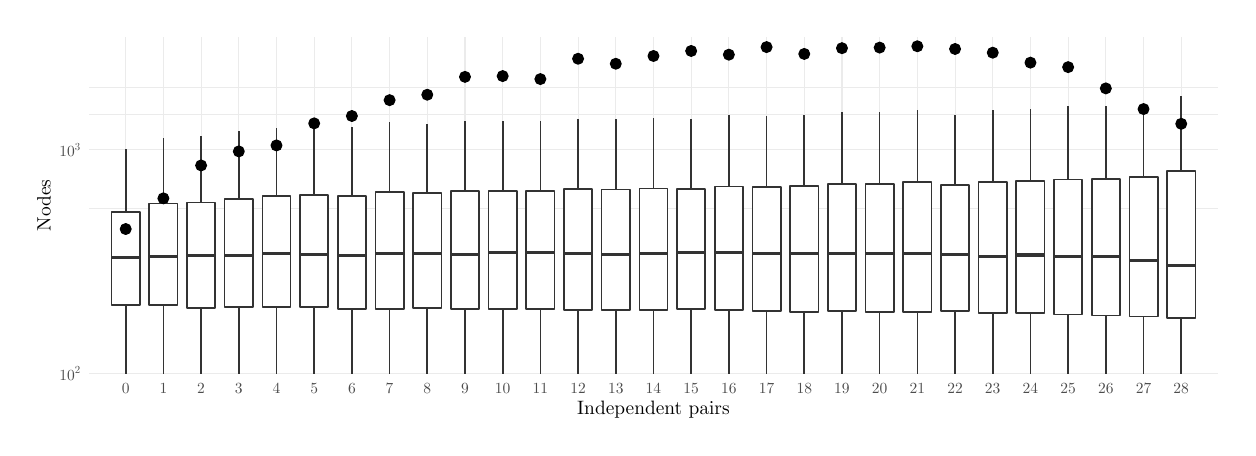
\begin{tikzpicture}[x=1pt,y=1pt]
\definecolor{fillColor}{RGB}{255,255,255}
\path[use as bounding box,fill=fillColor,fill opacity=0.00] (0,0) rectangle (433.62,144.54);
\begin{scope}
\path[clip] ( 22.14, 19.53) rectangle (430.12,141.04);
\definecolor{drawColor}{gray}{0.92}

\path[draw=drawColor,line width= 0.2pt,line join=round] ( 22.14, 79.39) --
	(430.12, 79.39);

\path[draw=drawColor,line width= 0.2pt,line join=round] ( 22.14,113.42) --
	(430.12,113.42);

\path[draw=drawColor,line width= 0.2pt,line join=round] ( 22.14,122.92) --
	(430.12,122.92);

\path[draw=drawColor,line width= 0.4pt,line join=round] ( 22.14, 19.53) --
	(430.12, 19.53);

\path[draw=drawColor,line width= 0.4pt,line join=round] ( 22.14,100.38) --
	(430.12,100.38);

\path[draw=drawColor,line width= 0.4pt,line join=round] ( 35.42, 19.53) --
	( 35.42,141.04);

\path[draw=drawColor,line width= 0.4pt,line join=round] ( 49.04, 19.53) --
	( 49.04,141.04);

\path[draw=drawColor,line width= 0.4pt,line join=round] ( 62.67, 19.53) --
	( 62.67,141.04);

\path[draw=drawColor,line width= 0.4pt,line join=round] ( 76.29, 19.53) --
	( 76.29,141.04);

\path[draw=drawColor,line width= 0.4pt,line join=round] ( 89.91, 19.53) --
	( 89.91,141.04);

\path[draw=drawColor,line width= 0.4pt,line join=round] (103.53, 19.53) --
	(103.53,141.04);

\path[draw=drawColor,line width= 0.4pt,line join=round] (117.15, 19.53) --
	(117.15,141.04);

\path[draw=drawColor,line width= 0.4pt,line join=round] (130.78, 19.53) --
	(130.78,141.04);

\path[draw=drawColor,line width= 0.4pt,line join=round] (144.40, 19.53) --
	(144.40,141.04);

\path[draw=drawColor,line width= 0.4pt,line join=round] (158.02, 19.53) --
	(158.02,141.04);

\path[draw=drawColor,line width= 0.4pt,line join=round] (171.64, 19.53) --
	(171.64,141.04);

\path[draw=drawColor,line width= 0.4pt,line join=round] (185.26, 19.53) --
	(185.26,141.04);

\path[draw=drawColor,line width= 0.4pt,line join=round] (198.89, 19.53) --
	(198.89,141.04);

\path[draw=drawColor,line width= 0.4pt,line join=round] (212.51, 19.53) --
	(212.51,141.04);

\path[draw=drawColor,line width= 0.4pt,line join=round] (226.13, 19.53) --
	(226.13,141.04);

\path[draw=drawColor,line width= 0.4pt,line join=round] (239.75, 19.53) --
	(239.75,141.04);

\path[draw=drawColor,line width= 0.4pt,line join=round] (253.37, 19.53) --
	(253.37,141.04);

\path[draw=drawColor,line width= 0.4pt,line join=round] (267.00, 19.53) --
	(267.00,141.04);

\path[draw=drawColor,line width= 0.4pt,line join=round] (280.62, 19.53) --
	(280.62,141.04);

\path[draw=drawColor,line width= 0.4pt,line join=round] (294.24, 19.53) --
	(294.24,141.04);

\path[draw=drawColor,line width= 0.4pt,line join=round] (307.86, 19.53) --
	(307.86,141.04);

\path[draw=drawColor,line width= 0.4pt,line join=round] (321.48, 19.53) --
	(321.48,141.04);

\path[draw=drawColor,line width= 0.4pt,line join=round] (335.11, 19.53) --
	(335.11,141.04);

\path[draw=drawColor,line width= 0.4pt,line join=round] (348.73, 19.53) --
	(348.73,141.04);

\path[draw=drawColor,line width= 0.4pt,line join=round] (362.35, 19.53) --
	(362.35,141.04);

\path[draw=drawColor,line width= 0.4pt,line join=round] (375.97, 19.53) --
	(375.97,141.04);

\path[draw=drawColor,line width= 0.4pt,line join=round] (389.59, 19.53) --
	(389.59,141.04);

\path[draw=drawColor,line width= 0.4pt,line join=round] (403.22, 19.53) --
	(403.22,141.04);

\path[draw=drawColor,line width= 0.4pt,line join=round] (416.84, 19.53) --
	(416.84,141.04);
\definecolor{drawColor}{gray}{0.20}

\path[draw=drawColor,line width= 0.6pt,line join=round] ( 35.42, 77.89) --
	( 35.42,100.83);

\path[draw=drawColor,line width= 0.6pt,line join=round] ( 35.42, 44.22) --
	( 35.42, 32.09) --
	( 35.42, 13.41) --
	( 35.42,  0.00);
\definecolor{fillColor}{RGB}{255,255,255}

\path[draw=drawColor,line width= 0.6pt,line join=round,line cap=round,fill=fillColor] ( 30.31, 77.89) --
	( 30.31, 44.22) --
	( 35.42, 44.22) --
	( 40.53, 44.22) --
	( 40.53, 77.89) --
	( 35.42, 77.89) --
	( 30.31, 77.89) --
	cycle;

\path[draw=drawColor,line width= 1.1pt,line join=round] ( 30.31, 61.34) --
	( 35.42, 61.34) --
	( 40.53, 61.34);

\path[draw=drawColor,line width= 0.6pt,line join=round] ( 49.04, 80.95) --
	( 49.04,104.79);

\path[draw=drawColor,line width= 0.6pt,line join=round] ( 49.04, 44.22) --
	( 49.04, 25.49) --
	( 49.04,  0.00);

\path[draw=drawColor,line width= 0.6pt,line join=round,line cap=round,fill=fillColor] ( 43.94, 80.95) --
	( 43.94, 44.22) --
	( 49.04, 44.22) --
	( 54.15, 44.22) --
	( 54.15, 80.95) --
	( 49.04, 80.95) --
	( 43.94, 80.95) --
	cycle;

\path[draw=drawColor,line width= 1.1pt,line join=round] ( 43.94, 61.98) --
	( 49.04, 61.98) --
	( 54.15, 61.98);

\path[draw=drawColor,line width= 0.6pt,line join=round] ( 62.67, 81.37) --
	( 62.67,105.47);

\path[draw=drawColor,line width= 0.6pt,line join=round] ( 62.67, 43.33) --
	( 62.67, 23.51) --
	( 62.67,  0.00);

\path[draw=drawColor,line width= 0.6pt,line join=round,line cap=round,fill=fillColor] ( 57.56, 81.37) --
	( 57.56, 43.33) --
	( 62.67, 43.33) --
	( 67.77, 43.33) --
	( 67.77, 81.37) --
	( 62.67, 81.37) --
	( 57.56, 81.37) --
	cycle;

\path[draw=drawColor,line width= 1.1pt,line join=round] ( 57.56, 62.29) --
	( 62.67, 62.29) --
	( 67.77, 62.29);

\path[draw=drawColor,line width= 0.6pt,line join=round] ( 76.29, 82.62) --
	( 76.29,107.07);

\path[draw=drawColor,line width= 0.6pt,line join=round] ( 76.29, 43.51) --
	( 76.29, 24.13) --
	( 76.29,  0.00);

\path[draw=drawColor,line width= 0.6pt,line join=round,line cap=round,fill=fillColor] ( 71.18, 82.62) --
	( 71.18, 43.51) --
	( 76.29, 43.51) --
	( 81.40, 43.51) --
	( 81.40, 82.62) --
	( 76.29, 82.62) --
	( 71.18, 82.62) --
	cycle;

\path[draw=drawColor,line width= 1.1pt,line join=round] ( 71.18, 62.29) --
	( 76.29, 62.29) --
	( 81.40, 62.29);

\path[draw=drawColor,line width= 0.6pt,line join=round] ( 89.91, 83.65) --
	( 89.91,108.35);

\path[draw=drawColor,line width= 0.6pt,line join=round] ( 89.91, 43.51) --
	( 89.91, 24.13) --
	( 89.91,  0.00);

\path[draw=drawColor,line width= 0.6pt,line join=round,line cap=round,fill=fillColor] ( 84.80, 83.65) --
	( 84.80, 43.51) --
	( 89.91, 43.51) --
	( 95.02, 43.51) --
	( 95.02, 83.65) --
	( 89.91, 83.65) --
	( 84.80, 83.65) --
	cycle;

\path[draw=drawColor,line width= 1.1pt,line join=round] ( 84.80, 63.01) --
	( 89.91, 63.01) --
	( 95.02, 63.01);

\path[draw=drawColor,line width= 0.6pt,line join=round] (103.53, 84.04) --
	(103.53,108.80);

\path[draw=drawColor,line width= 0.6pt,line join=round] (103.53, 43.69) --
	(103.53, 23.97) --
	(103.53,  0.00);

\path[draw=drawColor,line width= 0.6pt,line join=round,line cap=round,fill=fillColor] ( 98.42, 84.04) --
	( 98.42, 43.69) --
	(103.53, 43.69) --
	(108.64, 43.69) --
	(108.64, 84.04) --
	(103.53, 84.04) --
	( 98.42, 84.04) --
	cycle;

\path[draw=drawColor,line width= 1.1pt,line join=round] ( 98.42, 62.70) --
	(103.53, 62.70) --
	(108.64, 62.70);

\path[draw=drawColor,line width= 0.6pt,line join=round] (117.15, 83.71) --
	(117.15,108.60);

\path[draw=drawColor,line width= 0.6pt,line join=round] (117.15, 42.80) --
	(117.15, 23.51) --
	(117.15,  0.00);

\path[draw=drawColor,line width= 0.6pt,line join=round,line cap=round,fill=fillColor] (112.05, 83.71) --
	(112.05, 42.80) --
	(117.15, 42.80) --
	(122.26, 42.80) --
	(122.26, 83.71) --
	(117.15, 83.71) --
	(112.05, 83.71) --
	cycle;

\path[draw=drawColor,line width= 1.1pt,line join=round] (112.05, 62.29) --
	(117.15, 62.29) --
	(122.26, 62.29);

\path[draw=drawColor,line width= 0.6pt,line join=round] (130.78, 85.20) --
	(130.78,110.42);

\path[draw=drawColor,line width= 0.6pt,line join=round] (130.78, 42.80) --
	(130.78, 23.82) --
	(130.78,  0.00);

\path[draw=drawColor,line width= 0.6pt,line join=round,line cap=round,fill=fillColor] (125.67, 85.20) --
	(125.67, 42.80) --
	(130.78, 42.80) --
	(135.88, 42.80) --
	(135.88, 85.20) --
	(130.78, 85.20) --
	(125.67, 85.20) --
	cycle;

\path[draw=drawColor,line width= 1.1pt,line join=round] (125.67, 62.81) --
	(130.78, 62.81) --
	(135.88, 62.81);

\path[draw=drawColor,line width= 0.6pt,line join=round] (144.40, 84.71) --
	(144.40,109.70);

\path[draw=drawColor,line width= 0.6pt,line join=round] (144.40, 43.33) --
	(144.40, 24.74) --
	(144.40,  0.00);

\path[draw=drawColor,line width= 0.6pt,line join=round,line cap=round,fill=fillColor] (139.29, 84.71) --
	(139.29, 43.33) --
	(144.40, 43.33) --
	(149.51, 43.33) --
	(149.51, 84.71) --
	(144.40, 84.71) --
	(139.29, 84.71) --
	cycle;

\path[draw=drawColor,line width= 1.1pt,line join=round] (139.29, 62.91) --
	(144.40, 62.91) --
	(149.51, 62.91);

\path[draw=drawColor,line width= 0.6pt,line join=round] (158.02, 85.52) --
	(158.02,110.81);

\path[draw=drawColor,line width= 0.6pt,line join=round] (158.02, 42.80) --
	(158.02, 23.35) --
	(158.02,  0.00);

\path[draw=drawColor,line width= 0.6pt,line join=round,line cap=round,fill=fillColor] (152.91, 85.52) --
	(152.91, 42.80) --
	(158.02, 42.80) --
	(163.13, 42.80) --
	(163.13, 85.52) --
	(158.02, 85.52) --
	(152.91, 85.52) --
	cycle;

\path[draw=drawColor,line width= 1.1pt,line join=round] (152.91, 62.70) --
	(158.02, 62.70) --
	(163.13, 62.70);

\path[draw=drawColor,line width= 0.6pt,line join=round] (171.64, 85.52) --
	(171.64,110.65);

\path[draw=drawColor,line width= 0.6pt,line join=round] (171.64, 42.98) --
	(171.64, 30.84) --
	(171.64, 12.13) --
	(171.64,  0.00);

\path[draw=drawColor,line width= 0.6pt,line join=round,line cap=round,fill=fillColor] (166.53, 85.52) --
	(166.53, 42.98) --
	(171.64, 42.98) --
	(176.75, 42.98) --
	(176.75, 85.52) --
	(171.64, 85.52) --
	(166.53, 85.52) --
	cycle;

\path[draw=drawColor,line width= 1.1pt,line join=round] (166.53, 63.21) --
	(171.64, 63.21) --
	(176.75, 63.21);

\path[draw=drawColor,line width= 0.6pt,line join=round] (185.26, 85.63) --
	(185.26,110.94);

\path[draw=drawColor,line width= 0.6pt,line join=round] (185.26, 42.80) --
	(185.26, 23.82) --
	(185.26,  0.00);

\path[draw=drawColor,line width= 0.6pt,line join=round,line cap=round,fill=fillColor] (180.16, 85.63) --
	(180.16, 42.80) --
	(185.26, 42.80) --
	(190.37, 42.80) --
	(190.37, 85.63) --
	(185.26, 85.63) --
	(180.16, 85.63) --
	cycle;

\path[draw=drawColor,line width= 1.1pt,line join=round] (180.16, 63.21) --
	(185.26, 63.21) --
	(190.37, 63.21);

\path[draw=drawColor,line width= 0.6pt,line join=round] (198.89, 86.17) --
	(198.89,111.64);

\path[draw=drawColor,line width= 0.6pt,line join=round] (198.89, 42.61) --
	(198.89, 23.19) --
	(198.89,  0.00);

\path[draw=drawColor,line width= 0.6pt,line join=round,line cap=round,fill=fillColor] (193.78, 86.17) --
	(193.78, 42.61) --
	(198.89, 42.61) --
	(203.99, 42.61) --
	(203.99, 86.17) --
	(198.89, 86.17) --
	(193.78, 86.17) --
	cycle;

\path[draw=drawColor,line width= 1.1pt,line join=round] (193.78, 62.91) --
	(198.89, 62.91) --
	(203.99, 62.91);

\path[draw=drawColor,line width= 0.6pt,line join=round] (212.51, 86.11) --
	(212.51,111.59);

\path[draw=drawColor,line width= 0.6pt,line join=round] (212.51, 42.43) --
	(212.51, 23.35) --
	(212.51,  0.00);

\path[draw=drawColor,line width= 0.6pt,line join=round,line cap=round,fill=fillColor] (207.40, 86.11) --
	(207.40, 42.43) --
	(212.51, 42.43) --
	(217.62, 42.43) --
	(217.62, 86.11) --
	(212.51, 86.11) --
	(207.40, 86.11) --
	cycle;

\path[draw=drawColor,line width= 1.1pt,line join=round] (207.40, 62.50) --
	(212.51, 62.50) --
	(217.62, 62.50);

\path[draw=drawColor,line width= 0.6pt,line join=round] (226.13, 86.42) --
	(226.13,111.81);

\path[draw=drawColor,line width= 0.6pt,line join=round] (226.13, 42.61) --
	(226.13, 23.82) --
	(226.13,  0.00);

\path[draw=drawColor,line width= 0.6pt,line join=round,line cap=round,fill=fillColor] (221.02, 86.42) --
	(221.02, 42.61) --
	(226.13, 42.61) --
	(231.24, 42.61) --
	(231.24, 86.42) --
	(226.13, 86.42) --
	(221.02, 86.42) --
	cycle;

\path[draw=drawColor,line width= 1.1pt,line join=round] (221.02, 62.91) --
	(226.13, 62.91) --
	(231.24, 62.91);

\path[draw=drawColor,line width= 0.6pt,line join=round] (239.75, 86.32) --
	(239.75,111.71);

\path[draw=drawColor,line width= 0.6pt,line join=round] (239.75, 42.98) --
	(239.75, 24.13) --
	(239.75,  0.00);

\path[draw=drawColor,line width= 0.6pt,line join=round,line cap=round,fill=fillColor] (234.64, 86.32) --
	(234.64, 42.98) --
	(239.75, 42.98) --
	(244.86, 42.98) --
	(244.86, 86.32) --
	(239.75, 86.32) --
	(234.64, 86.32) --
	cycle;

\path[draw=drawColor,line width= 1.1pt,line join=round] (234.64, 63.21) --
	(239.75, 63.21) --
	(244.86, 63.21);

\path[draw=drawColor,line width= 0.6pt,line join=round] (253.37, 87.11) --
	(253.37,112.81);

\path[draw=drawColor,line width= 0.6pt,line join=round] (253.37, 42.43) --
	(253.37, 23.19) --
	(253.37,  0.00);

\path[draw=drawColor,line width= 0.6pt,line join=round,line cap=round,fill=fillColor] (248.27, 87.11) --
	(248.27, 42.43) --
	(253.37, 42.43) --
	(258.48, 42.43) --
	(258.48, 87.11) --
	(253.37, 87.11) --
	(248.27, 87.11) --
	cycle;

\path[draw=drawColor,line width= 1.1pt,line join=round] (248.27, 63.26) --
	(253.37, 63.26) --
	(258.48, 63.26);

\path[draw=drawColor,line width= 0.6pt,line join=round] (267.00, 87.00) --
	(267.00,112.67);

\path[draw=drawColor,line width= 0.6pt,line join=round] (267.00, 42.25) --
	(267.00, 23.82) --
	(267.00,  0.00);

\path[draw=drawColor,line width= 0.6pt,line join=round,line cap=round,fill=fillColor] (261.89, 87.00) --
	(261.89, 42.25) --
	(267.00, 42.25) --
	(272.10, 42.25) --
	(272.10, 87.00) --
	(267.00, 87.00) --
	(261.89, 87.00) --
	cycle;

\path[draw=drawColor,line width= 1.1pt,line join=round] (261.89, 62.91) --
	(267.00, 62.91) --
	(272.10, 62.91);

\path[draw=drawColor,line width= 0.6pt,line join=round] (280.62, 87.31) --
	(280.62,113.16);

\path[draw=drawColor,line width= 0.6pt,line join=round] (280.62, 41.88) --
	(280.62, 22.87) --
	(280.62,  0.00);

\path[draw=drawColor,line width= 0.6pt,line join=round,line cap=round,fill=fillColor] (275.51, 87.31) --
	(275.51, 41.88) --
	(280.62, 41.88) --
	(285.73, 41.88) --
	(285.73, 87.31) --
	(280.62, 87.31) --
	(275.51, 87.31) --
	cycle;

\path[draw=drawColor,line width= 1.1pt,line join=round] (275.51, 62.81) --
	(280.62, 62.81) --
	(285.73, 62.81);

\path[draw=drawColor,line width= 0.6pt,line join=round] (294.24, 88.10) --
	(294.24,113.98);

\path[draw=drawColor,line width= 0.6pt,line join=round] (294.24, 42.25) --
	(294.24, 23.19) --
	(294.24,  0.00);

\path[draw=drawColor,line width= 0.6pt,line join=round,line cap=round,fill=fillColor] (289.13, 88.10) --
	(289.13, 42.25) --
	(294.24, 42.25) --
	(299.35, 42.25) --
	(299.35, 88.10) --
	(294.24, 88.10) --
	(289.13, 88.10) --
	cycle;

\path[draw=drawColor,line width= 1.1pt,line join=round] (289.13, 63.01) --
	(294.24, 63.01) --
	(299.35, 63.01);

\path[draw=drawColor,line width= 0.6pt,line join=round] (307.86, 87.97) --
	(307.86,113.91);

\path[draw=drawColor,line width= 0.6pt,line join=round] (307.86, 41.88) --
	(307.86, 22.39) --
	(307.86,  0.00);

\path[draw=drawColor,line width= 0.6pt,line join=round,line cap=round,fill=fillColor] (302.75, 87.97) --
	(302.75, 41.88) --
	(307.86, 41.88) --
	(312.97, 41.88) --
	(312.97, 87.97) --
	(307.86, 87.97) --
	(302.75, 87.97) --
	cycle;

\path[draw=drawColor,line width= 1.1pt,line join=round] (302.75, 62.81) --
	(307.86, 62.81) --
	(312.97, 62.81);

\path[draw=drawColor,line width= 0.6pt,line join=round] (321.48, 88.70) --
	(321.48,114.80);

\path[draw=drawColor,line width= 0.6pt,line join=round] (321.48, 41.69) --
	(321.48, 22.39) --
	(321.48,  0.00);

\path[draw=drawColor,line width= 0.6pt,line join=round,line cap=round,fill=fillColor] (316.38, 88.70) --
	(316.38, 41.69) --
	(321.48, 41.69) --
	(326.59, 41.69) --
	(326.59, 88.70) --
	(321.48, 88.70) --
	(316.38, 88.70) --
	cycle;

\path[draw=drawColor,line width= 1.1pt,line join=round] (316.38, 62.81) --
	(321.48, 62.81) --
	(326.59, 62.81);

\path[draw=drawColor,line width= 0.6pt,line join=round] (335.11, 87.70) --
	(335.11,113.08);

\path[draw=drawColor,line width= 0.6pt,line join=round] (335.11, 42.06) --
	(335.11, 23.19) --
	(335.11,  0.00);

\path[draw=drawColor,line width= 0.6pt,line join=round,line cap=round,fill=fillColor] (330.00, 87.70) --
	(330.00, 42.06) --
	(335.11, 42.06) --
	(340.21, 42.06) --
	(340.21, 87.70) --
	(335.11, 87.70) --
	(330.00, 87.70) --
	cycle;

\path[draw=drawColor,line width= 1.1pt,line join=round] (330.00, 62.60) --
	(335.11, 62.60) --
	(340.21, 62.60);

\path[draw=drawColor,line width= 0.6pt,line join=round] (348.73, 88.75) --
	(348.73,114.92);

\path[draw=drawColor,line width= 0.6pt,line join=round] (348.73, 41.51) --
	(348.73, 22.55) --
	(348.73,  0.00);

\path[draw=drawColor,line width= 0.6pt,line join=round,line cap=round,fill=fillColor] (343.62, 88.75) --
	(343.62, 41.51) --
	(348.73, 41.51) --
	(353.84, 41.51) --
	(353.84, 88.75) --
	(348.73, 88.75) --
	(343.62, 88.75) --
	cycle;

\path[draw=drawColor,line width= 1.1pt,line join=round] (343.62, 61.98) --
	(348.73, 61.98) --
	(353.84, 61.98);

\path[draw=drawColor,line width= 0.6pt,line join=round] (362.35, 89.04) --
	(362.35,115.15);

\path[draw=drawColor,line width= 0.6pt,line join=round] (362.35, 41.32) --
	(362.35, 22.39) --
	(362.35,  0.00);

\path[draw=drawColor,line width= 0.6pt,line join=round,line cap=round,fill=fillColor] (357.24, 89.04) --
	(357.24, 41.32) --
	(362.35, 41.32) --
	(367.46, 41.32) --
	(367.46, 89.04) --
	(362.35, 89.04) --
	(357.24, 89.04) --
	cycle;

\path[draw=drawColor,line width= 1.1pt,line join=round] (357.24, 62.39) --
	(362.35, 62.39) --
	(367.46, 62.39);

\path[draw=drawColor,line width= 0.6pt,line join=round] (375.97, 89.66) --
	(375.97,116.10);

\path[draw=drawColor,line width= 0.6pt,line join=round] (375.97, 40.94) --
	(375.97, 22.87) --
	(375.97,  0.00);

\path[draw=drawColor,line width= 0.6pt,line join=round,line cap=round,fill=fillColor] (370.86, 89.66) --
	(370.86, 73.15) --
	(370.86, 40.94) --
	(375.97, 40.94) --
	(381.08, 40.94) --
	(381.08, 73.15) --
	(381.08, 89.66) --
	(375.97, 89.66) --
	(370.86, 89.66) --
	cycle;

\path[draw=drawColor,line width= 1.1pt,line join=round] (370.86, 61.98) --
	(375.97, 61.98) --
	(381.08, 61.98);

\path[draw=drawColor,line width= 0.6pt,line join=round] (389.59, 89.81) --
	(389.59,116.33);

\path[draw=drawColor,line width= 0.6pt,line join=round] (389.59, 40.55) --
	(389.59, 21.41) --
	(389.59,  0.00);

\path[draw=drawColor,line width= 0.6pt,line join=round,line cap=round,fill=fillColor] (384.49, 89.81) --
	(384.49, 73.19) --
	(384.49, 40.55) --
	(389.59, 40.55) --
	(394.70, 40.55) --
	(394.70, 73.19) --
	(394.70, 89.81) --
	(389.59, 89.81) --
	(384.49, 89.81) --
	cycle;

\path[draw=drawColor,line width= 1.1pt,line join=round] (384.49, 61.77) --
	(389.59, 61.77) --
	(394.70, 61.77);

\path[draw=drawColor,line width= 0.6pt,line join=round] (403.22, 90.61) --
	(403.22,117.36);

\path[draw=drawColor,line width= 0.6pt,line join=round] (403.22, 40.17) --
	(403.22, 21.57) --
	(403.22,  0.00);

\path[draw=drawColor,line width= 0.6pt,line join=round,line cap=round,fill=fillColor] (398.11, 90.61) --
	(398.11, 73.76) --
	(398.11, 40.17) --
	(403.22, 40.17) --
	(408.32, 40.17) --
	(408.32, 73.76) --
	(408.32, 90.61) --
	(403.22, 90.61) --
	(398.11, 90.61) --
	cycle;

\path[draw=drawColor,line width= 1.1pt,line join=round] (398.11, 60.26) --
	(403.22, 60.26) --
	(408.32, 60.26);

\path[draw=drawColor,line width= 0.6pt,line join=round] (416.84, 92.67) --
	(416.84,119.87);

\path[draw=drawColor,line width= 0.6pt,line join=round] (416.84, 39.58) --
	(416.84, 20.74) --
	(416.84,  0.00);

\path[draw=drawColor,line width= 0.6pt,line join=round,line cap=round,fill=fillColor] (411.73, 92.67) --
	(411.73, 75.33) --
	(411.73, 39.58) --
	(416.84, 39.58) --
	(421.95, 39.58) --
	(421.95, 75.33) --
	(421.95, 92.67) --
	(416.84, 92.67) --
	(411.73, 92.67) --
	cycle;

\path[draw=drawColor,line width= 1.1pt,line join=round] (411.73, 58.57) --
	(416.84, 58.57) --
	(421.95, 58.57);
\definecolor{drawColor}{RGB}{0,0,0}
\definecolor{fillColor}{RGB}{0,0,0}

\path[draw=drawColor,line width= 0.4pt,line join=round,line cap=round,fill=fillColor] ( 35.42, 71.78) circle (  1.96);

\path[draw=drawColor,line width= 0.4pt,line join=round,line cap=round,fill=fillColor] ( 49.04, 82.87) circle (  1.96);

\path[draw=drawColor,line width= 0.4pt,line join=round,line cap=round,fill=fillColor] ( 62.67, 94.76) circle (  1.96);

\path[draw=drawColor,line width= 0.4pt,line join=round,line cap=round,fill=fillColor] ( 76.29, 99.83) circle (  1.96);

\path[draw=drawColor,line width= 0.4pt,line join=round,line cap=round,fill=fillColor] ( 89.91,101.99) circle (  1.96);

\path[draw=drawColor,line width= 0.4pt,line join=round,line cap=round,fill=fillColor] (103.53,109.96) circle (  1.96);

\path[draw=drawColor,line width= 0.4pt,line join=round,line cap=round,fill=fillColor] (117.15,112.62) circle (  1.96);

\path[draw=drawColor,line width= 0.4pt,line join=round,line cap=round,fill=fillColor] (130.78,118.35) circle (  1.96);

\path[draw=drawColor,line width= 0.4pt,line join=round,line cap=round,fill=fillColor] (144.40,120.31) circle (  1.96);

\path[draw=drawColor,line width= 0.4pt,line join=round,line cap=round,fill=fillColor] (158.02,126.76) circle (  1.96);

\path[draw=drawColor,line width= 0.4pt,line join=round,line cap=round,fill=fillColor] (171.64,127.05) circle (  1.96);

\path[draw=drawColor,line width= 0.4pt,line join=round,line cap=round,fill=fillColor] (185.26,125.96) circle (  1.96);

\path[draw=drawColor,line width= 0.4pt,line join=round,line cap=round,fill=fillColor] (198.89,133.31) circle (  1.96);

\path[draw=drawColor,line width= 0.4pt,line join=round,line cap=round,fill=fillColor] (212.51,131.50) circle (  1.96);

\path[draw=drawColor,line width= 0.4pt,line join=round,line cap=round,fill=fillColor] (226.13,134.31) circle (  1.96);

\path[draw=drawColor,line width= 0.4pt,line join=round,line cap=round,fill=fillColor] (239.75,136.12) circle (  1.96);

\path[draw=drawColor,line width= 0.4pt,line join=round,line cap=round,fill=fillColor] (253.37,134.78) circle (  1.96);

\path[draw=drawColor,line width= 0.4pt,line join=round,line cap=round,fill=fillColor] (267.00,137.52) circle (  1.96);

\path[draw=drawColor,line width= 0.4pt,line join=round,line cap=round,fill=fillColor] (280.62,135.05) circle (  1.96);

\path[draw=drawColor,line width= 0.4pt,line join=round,line cap=round,fill=fillColor] (294.24,137.13) circle (  1.96);

\path[draw=drawColor,line width= 0.4pt,line join=round,line cap=round,fill=fillColor] (307.86,137.34) circle (  1.96);

\path[draw=drawColor,line width= 0.4pt,line join=round,line cap=round,fill=fillColor] (321.48,137.82) circle (  1.96);

\path[draw=drawColor,line width= 0.4pt,line join=round,line cap=round,fill=fillColor] (335.11,136.84) circle (  1.96);

\path[draw=drawColor,line width= 0.4pt,line join=round,line cap=round,fill=fillColor] (348.73,135.50) circle (  1.96);

\path[draw=drawColor,line width= 0.4pt,line join=round,line cap=round,fill=fillColor] (362.35,131.90) circle (  1.96);

\path[draw=drawColor,line width= 0.4pt,line join=round,line cap=round,fill=fillColor] (375.97,130.28) circle (  1.96);

\path[draw=drawColor,line width= 0.4pt,line join=round,line cap=round,fill=fillColor] (389.59,122.60) circle (  1.96);

\path[draw=drawColor,line width= 0.4pt,line join=round,line cap=round,fill=fillColor] (403.22,115.13) circle (  1.96);

\path[draw=drawColor,line width= 0.4pt,line join=round,line cap=round,fill=fillColor] (416.84,109.80) circle (  1.96);
\end{scope}
\begin{scope}
\path[clip] (  0.00,  0.00) rectangle (433.62,144.54);
\definecolor{drawColor}{gray}{0.30}

\node[text=drawColor,anchor=base west,inner sep=0pt, outer sep=0pt, scale=  0.56] at ( 11.43, 17.12) {10};

\node[text=drawColor,anchor=base west,inner sep=0pt, outer sep=0pt, scale=  0.39] at ( 17.03, 19.41) {2};

\node[text=drawColor,anchor=base west,inner sep=0pt, outer sep=0pt, scale=  0.56] at ( 11.43, 97.98) {10};

\node[text=drawColor,anchor=base west,inner sep=0pt, outer sep=0pt, scale=  0.39] at ( 17.03,100.27) {3};
\end{scope}
\begin{scope}
\path[clip] (  0.00,  0.00) rectangle (433.62,144.54);
\definecolor{drawColor}{gray}{0.30}

\node[text=drawColor,anchor=base,inner sep=0pt, outer sep=0pt, scale=  0.56] at ( 35.42, 12.52) {0};

\node[text=drawColor,anchor=base,inner sep=0pt, outer sep=0pt, scale=  0.56] at ( 49.04, 12.52) {1};

\node[text=drawColor,anchor=base,inner sep=0pt, outer sep=0pt, scale=  0.56] at ( 62.67, 12.52) {2};

\node[text=drawColor,anchor=base,inner sep=0pt, outer sep=0pt, scale=  0.56] at ( 76.29, 12.52) {3};

\node[text=drawColor,anchor=base,inner sep=0pt, outer sep=0pt, scale=  0.56] at ( 89.91, 12.52) {4};

\node[text=drawColor,anchor=base,inner sep=0pt, outer sep=0pt, scale=  0.56] at (103.53, 12.52) {5};

\node[text=drawColor,anchor=base,inner sep=0pt, outer sep=0pt, scale=  0.56] at (117.15, 12.52) {6};

\node[text=drawColor,anchor=base,inner sep=0pt, outer sep=0pt, scale=  0.56] at (130.78, 12.52) {7};

\node[text=drawColor,anchor=base,inner sep=0pt, outer sep=0pt, scale=  0.56] at (144.40, 12.52) {8};

\node[text=drawColor,anchor=base,inner sep=0pt, outer sep=0pt, scale=  0.56] at (158.02, 12.52) {9};

\node[text=drawColor,anchor=base,inner sep=0pt, outer sep=0pt, scale=  0.56] at (171.64, 12.52) {10};

\node[text=drawColor,anchor=base,inner sep=0pt, outer sep=0pt, scale=  0.56] at (185.26, 12.52) {11};

\node[text=drawColor,anchor=base,inner sep=0pt, outer sep=0pt, scale=  0.56] at (198.89, 12.52) {12};

\node[text=drawColor,anchor=base,inner sep=0pt, outer sep=0pt, scale=  0.56] at (212.51, 12.52) {13};

\node[text=drawColor,anchor=base,inner sep=0pt, outer sep=0pt, scale=  0.56] at (226.13, 12.52) {14};

\node[text=drawColor,anchor=base,inner sep=0pt, outer sep=0pt, scale=  0.56] at (239.75, 12.52) {15};

\node[text=drawColor,anchor=base,inner sep=0pt, outer sep=0pt, scale=  0.56] at (253.37, 12.52) {16};

\node[text=drawColor,anchor=base,inner sep=0pt, outer sep=0pt, scale=  0.56] at (267.00, 12.52) {17};

\node[text=drawColor,anchor=base,inner sep=0pt, outer sep=0pt, scale=  0.56] at (280.62, 12.52) {18};

\node[text=drawColor,anchor=base,inner sep=0pt, outer sep=0pt, scale=  0.56] at (294.24, 12.52) {19};

\node[text=drawColor,anchor=base,inner sep=0pt, outer sep=0pt, scale=  0.56] at (307.86, 12.52) {20};

\node[text=drawColor,anchor=base,inner sep=0pt, outer sep=0pt, scale=  0.56] at (321.48, 12.52) {21};

\node[text=drawColor,anchor=base,inner sep=0pt, outer sep=0pt, scale=  0.56] at (335.11, 12.52) {22};

\node[text=drawColor,anchor=base,inner sep=0pt, outer sep=0pt, scale=  0.56] at (348.73, 12.52) {23};

\node[text=drawColor,anchor=base,inner sep=0pt, outer sep=0pt, scale=  0.56] at (362.35, 12.52) {24};

\node[text=drawColor,anchor=base,inner sep=0pt, outer sep=0pt, scale=  0.56] at (375.97, 12.52) {25};

\node[text=drawColor,anchor=base,inner sep=0pt, outer sep=0pt, scale=  0.56] at (389.59, 12.52) {26};

\node[text=drawColor,anchor=base,inner sep=0pt, outer sep=0pt, scale=  0.56] at (403.22, 12.52) {27};

\node[text=drawColor,anchor=base,inner sep=0pt, outer sep=0pt, scale=  0.56] at (416.84, 12.52) {28};
\end{scope}
\begin{scope}
\path[clip] (  0.00,  0.00) rectangle (433.62,144.54);
\definecolor{drawColor}{RGB}{0,0,0}

\node[text=drawColor,anchor=base,inner sep=0pt, outer sep=0pt, scale=  0.70] at (226.13,  4.86) {Independent pairs};
\end{scope}
\begin{scope}
\path[clip] (  0.00,  0.00) rectangle (433.62,144.54);
\definecolor{drawColor}{RGB}{0,0,0}

\node[text=drawColor,rotate= 90.00,anchor=base,inner sep=0pt, outer sep=0pt, scale=  0.70] at (  8.32, 80.28) {Nodes};
\end{scope}
\end{tikzpicture}
}
  \end{figure}
\end{frame}

\section{WMC}

\begin{frame}{Defining WMC}
  \begin{definition}
    Let $\mathbf{B}$ be an atomic Boolean algebra. Let $L \subset \mathbf{B}$ be
    such that every atom $m$ can be uniquely expressed as $m = \bigwedge L'$ for
    some $L' \subseteq L$, and let $w\colon L \to \mathbb{R}_{\ge 0}$ be
    arbitrary. The \alert{weighted model count} $\mathsf{WMC}_w\colon \mathbf{B}
    \to \mathbb{R}_{\ge 0}$ is defined as
    \[
      \mathsf{WMC}_w(x) = \begin{cases}
        0 & \text{if } x = 0 \\
        \prod_{l \in L'} w(l) & \text{if } x = \bigwedge L' \text{ is an atom}
        \\
        \sum_{\text{atoms } a \le x} \mathsf{WMC}_w(a) & \text{otherwise}
      \end{cases}
    \]
    for any $x \in \mathbf{B}$.
  \end{definition}
\end{frame}

\begin{frame}{WMC Requires Independent Literals}
  \begin{theorem}
    Let $\mathbf{B}$ be a free Boolean algebra over $\{ l_i \}_{i=1}^n$ with
    measure
    \[
      m\colon \mathbf{B} \to \mathbb{R}_{\ge 0},
    \]
    and let
    \[
      L = \{ l_i \}_{i = 1}^n \cup \{\neg l_i \}_{i = 1}^n.
    \]
    Then there exists a weight function $w\colon L \to \mathbb{R}_{\ge 0}$ such
    that $m = \mathsf{WMC}_w$ if and only if
    \[
      m(l \land l') = m(l)m(l')
    \]
    for all distinct $l, l' \in L$ such that $l \ne \neg l'$.
  \end{theorem}
\end{frame}

\begin{frame}[fragile]{Extending the Algebra}
  \[
    \begin{tikzcd}
      \textcolor{red}{\mathbb{R}_{\ge 0}} & & \\
      \textcolor{red}{\mathbf{B}} \arrow[red]{u}{m} \ar[r,hookrightarrow,"\iota"]
      & \mathbf{B'} \arrow{lu}[swap]{m'} & \\
      \textcolor{red}{L} \ar[u,red,hookrightarrow] \ar[r,hookrightarrow] & L'
      \ar[u,hookrightarrow] \arrow{r}{w} & \mathbb{R}_{\ge 0}
    \end{tikzcd}
  \]
\end{frame}

\begin{frame}{How Can This Benefit Inference?}
  \begin{theorem}[\cite{sikorski1969boolean}]
    If $\mathbf{B} = \mathcal{F}\{a\} + \mathcal{F}\{b\}$, then $\Pr(a \land b) =
    \Pr(a)\Pr(b)$.
  \end{theorem}
  \pause
  \begin{conjecture}
    If $\mathbf{B} = \mathcal{F}\{a\} +_{\mathcal{F}\{c\}} \mathcal{F}\{b\}$, then $\Pr(a
    \land b \land c) = \Pr(a \land c)\Pr(b \land c)$.
  \end{conjecture}
  \pause
  \begin{conjecture}
    Using coproducts and pushouts, one can encode a Bayesian network into WMC
    with \alert{fewer literals} and a \alert{shorter theory} than before.
  \end{conjecture}
  \pause
  \begin{conjecture}
    A \#\SAT{} algorithm can be adapted without sacrificing efficiency.
  \end{conjecture}
\end{frame}

\section{Future Work}

\begin{frame}[fragile]{Abstraction: Before}
  \[
    \begin{tikzcd}[column sep=tiny]
      \colorbox{color7}{Theory $\Delta_h$} & \colorbox{color7}{Constants}
      \arrow{d}[swap]{\colorbox{color7}{Predicates}} & & \colorbox{color7}{Constants}
      \arrow{d}{\colorbox{color7}{Predicates}} & \colorbox{color7}{Theory $\Delta_l$} \\
      & \text{Atoms} \ar[d,hookrightarrow]
      \arrow[rrdd,"\mathrm{Refinement}"{sloped}] & & \text{Atoms}
      \ar[d,hookrightarrow] & \\
      \mathbb{R}_{\ge 0} & \text{Literals} \arrow{l}[swap]{\colorbox{color7}{$w_h$}}
      \ar[d,hookrightarrow] & & \text{Literals} \arrow{r}{\colorbox{color7}{$w_l$}}
      \ar[d,hookrightarrow] & \mathbb{R}_{\ge 0} \\
      & \text{Formulas} \arrow{rd}[swap]{\Pr} \arrow[loop left, "\land{,}
      \lor{,} \neg"] & & \text{Formulas} \arrow{ld}{\Pr} \arrow[loop right,
      "\land{,} \lor{,} \neg"] & \\
      & & \left[ 0, 1 \right] & &
    \end{tikzcd}
  \]
\end{frame}

\begin{frame}[fragile]{Abstraction: After}
  \[
    \begin{tikzcd}
      S_h \ar[d,hookrightarrow] \ar[rd] & S_l \ar[d,hookrightarrow] \\
      \mathbf{B}_h \ar[d] \ar[r,dashed] & \mathbf{B}_l \ar[d] \\
      \mathbf{B}_h/(\neg\Delta_h) \ar[r,dashed] & \mathbf{B}_l/(\neg\Delta_l)
    \end{tikzcd}
  \]
\end{frame}

\begin{frame}{Reflections \& Future Work}
  \begin{itemize}
  \item The equivalence paper needs significant rework.
  \item The program generation paper could be improved by demonstrating the
    model's usefulness.
  \item The WMC paper needs successful experimental results.
  \item Understanding PRMs as algebras is promising---in one way or another.
  \end{itemize}
\end{frame}

\end{document}